%%%%%%%%%%%%%%%%%%%%%%%%%%%%%%%%%%%%%%%%%%%%%%%%%%%%%%%%%%%%
% Dokument-Einstellungen
\documentclass{SMBV12}

%%%%%%%%%%%%%%%%%%%%%%%%%%%%%%%%%%%%%%%%%%%%%%%%%%%%%%%%%%%%
%-----------------------------------------------------------
% Hier beginnt das eigentliche Dokument
\begin{document}

\title{Graph-Based Segmentation}

\author{Phan-Anh Nguyen}

\maketitle

%%%%%%%%%%%%%%%%%%%%%%%%%%%%%%%%%%%%%%%%%%%%%%%%%%%%%%%%%%%%
%-----------------------------------------------------------% Zusammenfassung

\begin{abstract}%
Abstract. This 20-page seminar paper reviews state-of-the-art graph-based segmentation algorithms.
\end{abstract}

\keywords{Proceedings, Graph Cut, Segmentation}


%%%%%%%%%%%%%%%%%%%%%%%%%%%%%%%%%%%%%%%%%%%%%%%%%%%%%%%%%%%%
%-----------------------------------------------------------
%
\section{Introduction}

Introduction is written last.



%%%%%%%%%%%%%%%%%%%%%%%%%%%%%%%%%%%%%%%%%%%%%%%%%%%%%%%%%%%%
%-----------------------------------------------------------
%
\section{Image Features}


%%%%%%%%%%%%%%%%%%%%%%%%%%%%%%%%%%%%%%%%%%%%%%%%%%%%%%%%%%%%
\subsection{Image Feature Overview}

What are image features? How can we describe/represent them?


%%%%%%%%%%%%%%%%%%%%%%%%%%%%%%%%%%%%%%%%%%%%%%%%%%%%%%%%%%%%
\subsection{SURF descriptor}




%%%%%%%%%%%%%%%%%%%%%%%%%%%%%%%%%%%%%%%%%%%%%%%%%%%%%%%%%%%%
\subsection{Edges and Contours}


\begin{itemize}
\item
	Edges
\item
	Contours
\end{itemize}


%%%%%%%%%%%%%%%%%%%%%%%%%%%%%%%%%%%%%%%%%%%%%%%%%%%%%%%%%%%%
\subsection{}



%%%%%%%%%%%%%%%%%%%%%%%%%%%%%%%%%%%%%%%%%%%%%%%%%%%%%%%%%%%%
\subsection{}


{\em emphasize}.

%%%%%%%%%%%%%%%%%%%%%%%%%%%%%%%%%%%%%%%%%%%%%%%%%%%%%%%%%%%%
\subsection{}

{\em subfigure}  (\figurename~\ref{SMBV12_EMuster_fig01}).

\begin{figure}[b]
 	\centering
		\subfigure[Eins]{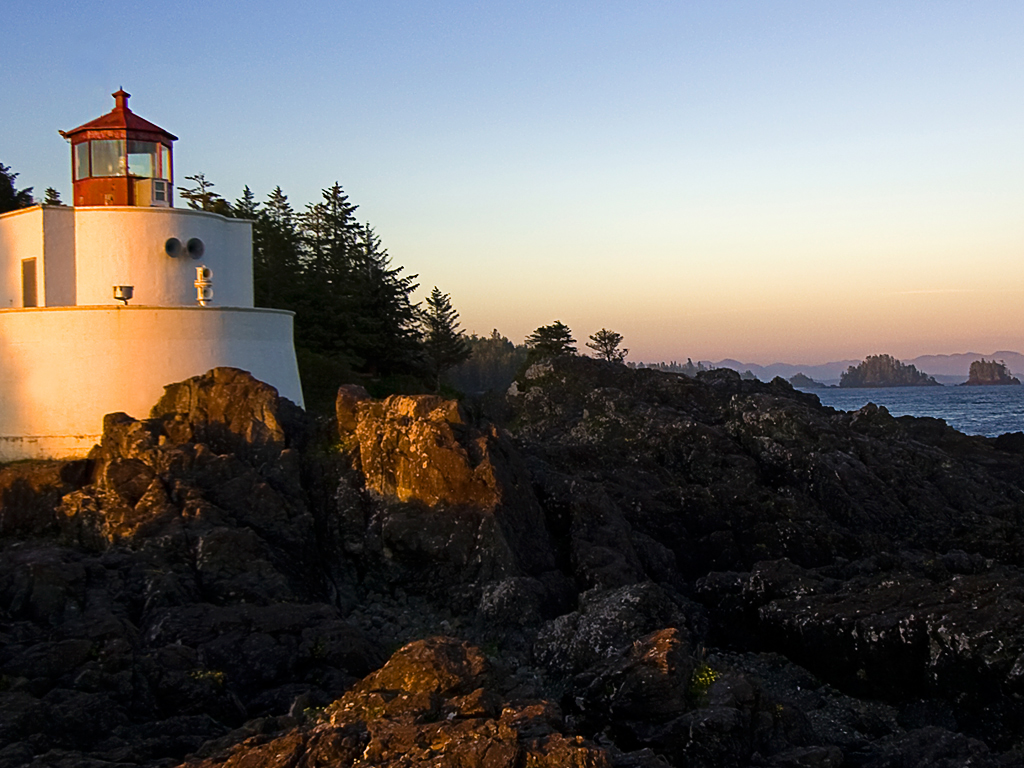
\includegraphics[width=0.3\textwidth]{Images/Lighthouse.jpg}}
		\subfigure[Zwei]{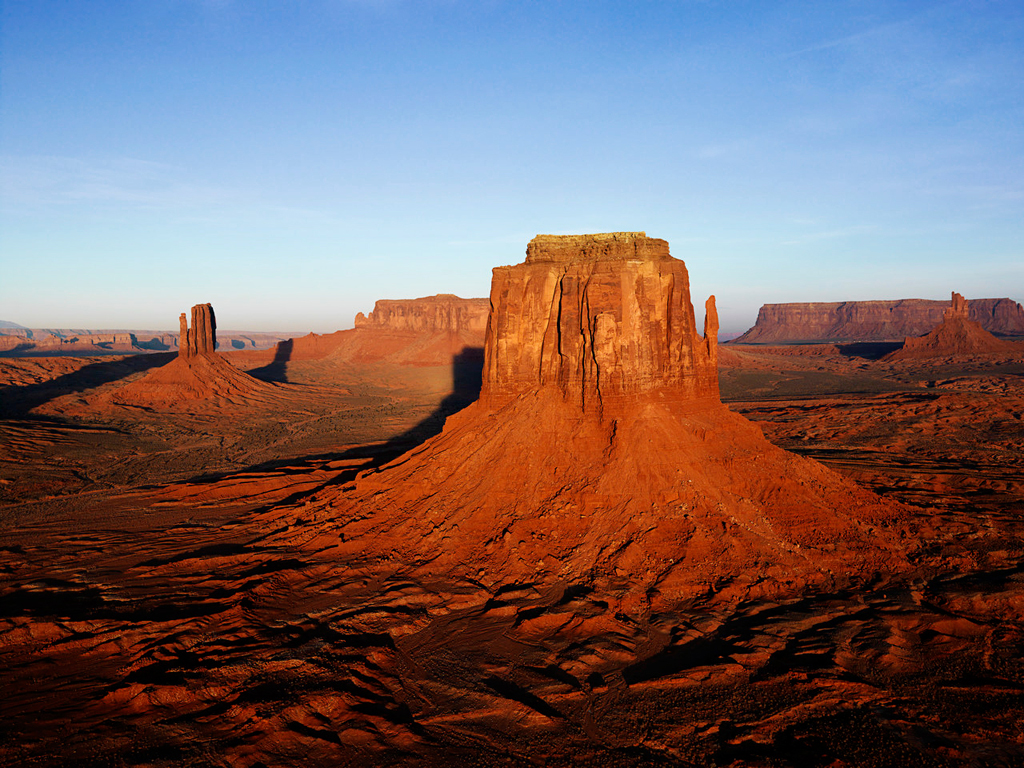
\includegraphics[width=0.3\textwidth]{Images/Desert.jpg}}
		\subfigure[Drei]{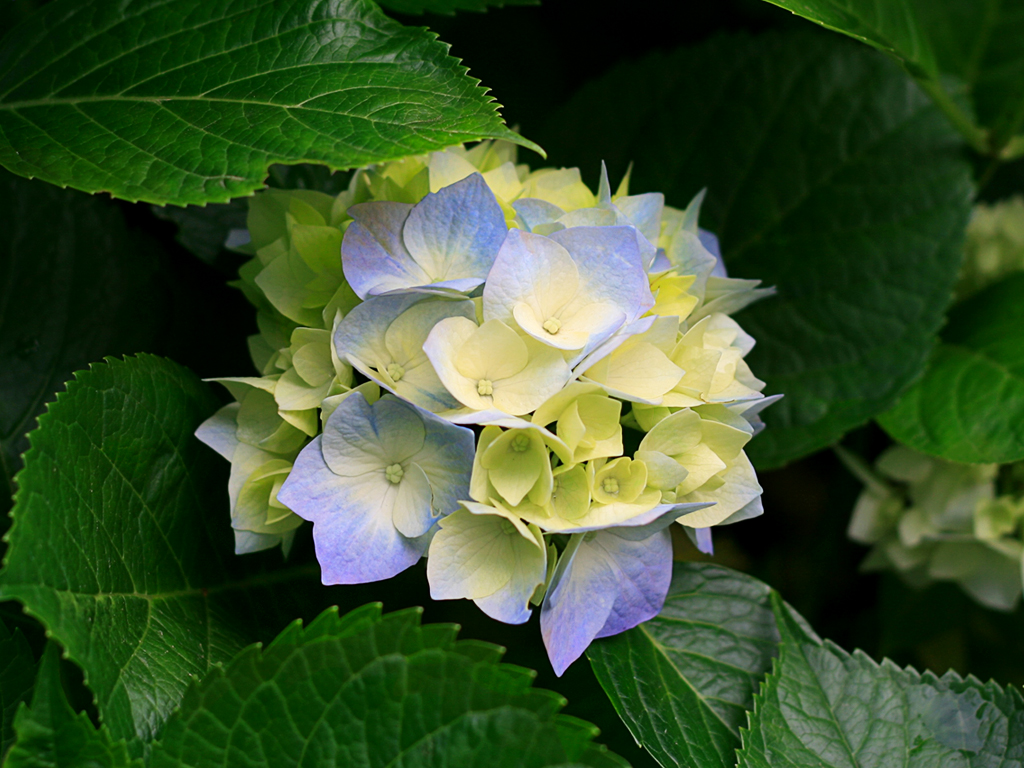
\includegraphics[width=0.3\textwidth]{Images/Hydrangeas.jpg}}
 		\caption{\label{SMBV12_EMuster_fig01} Example.}
\end{figure}

%%%%%%%%%%%%%%%%%%%%%%%%%%%%%%%%%%%%%%%%%%%%%%%%%%%%%%%%%%%%
\subsection{}






%%%%%%%%%%%%%%%%%%%%%%%%%%%%%%%%%%%%%%%%%%%%%%%%%%%%%%%%%%%%
\subsection{}


\begin{equation}
c=sqrt(a^2+b^2)
\end{equation}
$x+y=z$.


%%%%%%%%%%%%%%%%%%%%%%%%%%%%%%%%%%%%%%%%%%%%%%%%%%%%%%%%%%%%
\subsection{}




%%%%%%%%%%%%%%%%%%%%%%%%%%%%%%%%%%%%%%%%%%%%%%%%%%%%%%%%%%%%
\subsection{Literaturangaben}

\cite{Rut84}.
\nobreak{\tt http://www.library.uq.edu.au/training/citation/vancouv.pdf}.

%%%%%%%%%%%%%%%%%%%%%%%%%%%%%%%%%%%%%%%%%%%%%%%%%%%%%%%%%%%%
\subsection{}



\section{}



\section{}



%%%%%%%%%%%%%%%%%%%%%%%%%%%%%%%%%%%%%%%%%%%%%%%%%%%%%%%%%%%%
%-----------------------------------------------------------
%
\def\refname{Literature}
\begin{thebibliography}{AA}


\bibitem {Rut84} Ruttimann UE, Groenhuis RAJ, Webber RL:
                 Restoration of digital multiplane tomosynthesis by a
                 constrained iteration method.
                 IEEE Trans. on Medical Imaging, 1984;
                 3(3): 141--148.

\bibitem {Ebe76} Ebert H (Hrsg.):
                 Physikalisches Taschenbuch.
                 Vieweg Verlag, Braunschweig, 5.\ Auflage 1976.

\end{thebibliography}

\noindent
\begin{picture}(160,242)
\put(0,0){\framebox(160,242){}}
\end{picture}

\end{document}
